\documentclass{article}
\usepackage{graphicx}
\usepackage{epsfig,epstopdf}
\usepackage{amssymb,amsmath,bm}
\usepackage{textcomp}
\usepackage{caption}
\usepackage{multirow}
\usepackage{nonfloat}
\usepackage{flushend}
%\usepackage{subfigure}
\usepackage{algorithm}
\usepackage{subcaption}
\usepackage{algorithmic}
\usepackage{url}
\usepackage{hyperref}
\usepackage{lipsum}

\DeclareMathSizes{10}{10}{10}{10}




\title{NLP Project Report}

\author{ {\bf Group 13} \\ \vspace{4mm} Saranya .M .S (CS15D006), Sridharan Sankaran (CS14S024)}

\begin{document}
\maketitle

\section*{Project title}
{ \textit {Weather/Cyclone forecast using NLG techniques}}

\section*{Problem Definition}
$\quad \; $ In this project work, a weather report is generated to forecast the climatic conditions and cyclone warnings from the satellite images using image processing, data mining and Natural Language Generation techniques in a conversational language instead of telegraphic-weather-language. A text-to-speech synthesis system is used to read the report using synthesized voice. The navigation direction of cyclone is predicted after processing the satellite images. 

The forecast is not only made for the cyclone warnings but also for forecasting daily weather conditions. The location of the cyclone is given with respect to the near-by cities for easy readability.
A look-up table with  list of near-by cities along with their latitude and longitudinal values is used for this purpose. The trajectory of the cyclone is also calculated based on the direction and speed of the cyclones along with the nearby target cities. A 5-day weather forecast is made with the time-series of various weather parameters over a period of 5 days given by an open weather API. Then a text to speech synthesis system is implemented using HMM based speech synthesis system to read this text report for visually challenged people. 

\newpage
\vspace{-3cm}
\section{Introduction}
\label{sec:intro}
Weather forecasting become an essential thing in our daily life to know the upcoming 
natural calamities. With the advancement in the meteorology and communication 
technology, images obtained by the satellites stationed above are used in weather
forecasting. But the forecasting requires intense training and advanced education to 
interpret the information form the satellite pictures. Meteorological department has already
automated the gathering of satellite images in the database. Further advancement can be
brought by automating the weather forecasting. Although the automated forecast may not
be as accurate as the experts interpretation \cite{weatherReport}, Forecast Production Assistant (FPA) was 
developed to automate the routine aspects for public health and safety in hazardous
 weather \cite{fpa}. 

\vspace{-2mm}
\section{Input sources}
\label{sec:db}
Two types of input data are required to forecast the weather report. For cyclone forecast, satellite images are needed and for daily weather forecast other weather parameters like rain, wind, humidity etc are needed. The source of these data-sets are given in the subsections below.

\subsection{Image database}
\label{ssec:imgDB}
The satellite images are gathered from Hong kong Observatory website located at $http://www.hko.gov.hk/wxinfo/intersat/satellite/sate.htm$. Here we consider deep convection weather images of Asia taken from satellites at intervals of about once every half-hour. Deep convection clouds are very dense with water content and  are seen as red patches in the images. The sample satellite image used for cyclone forecast is shown in the Figure~\ref{fig:cyclone}.

\begin{figure}[h!tb]
\centering
\includegraphics[scale=0.18]{figures/cyclone.png}
\caption{Satellite image of a cyclone}
\label{fig:cyclone}
\end{figure}

\clearpage

\subsection{Weather parameters}
\label{ssec:weatherParams}
For preparing the 5-day weather forecast report, the weather parameters are collected from $www.openweathermap.org$ using an API. This site will have the information of atmospheric changes for every 3 hours as shown in the Figure~\ref{fig:sampleData}.

\begin{figure}[h!tb]
\centering
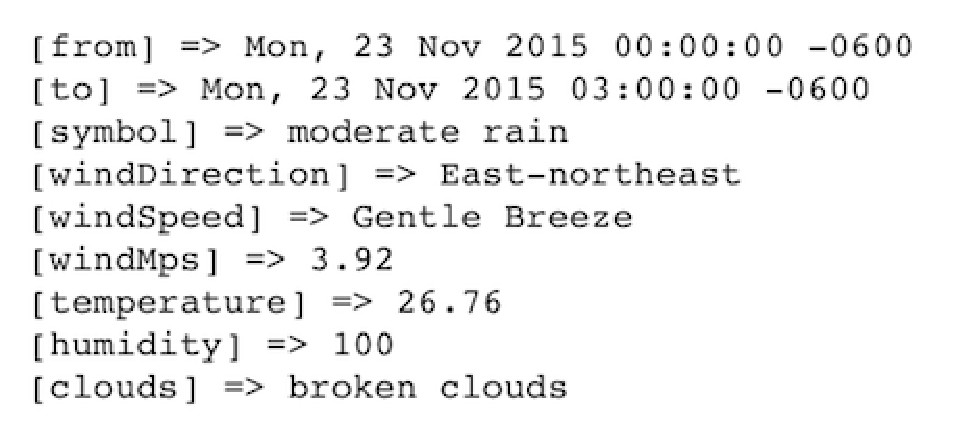
\includegraphics[scale=0.5]{figures/weatherData.eps}
\caption{Sample weather parameters}
\label{fig:sampleData}
\end{figure}

\subsection{Speech corpus}
\label{ssec:speechCorpus}

For developing a TTS system, we need the recorded speech content, generally called
as speech corpus which serves as a database. The text-to-Speech synthesis process needs
two types of data namely, 1) Text data and 2) Speech data. The former one is the text
form of the content which is to be recorded to get the later form of data. Here for the 
purpose of developing a phoneme-based speech synthesis model of English language, one
hour of CMU-artic corpus is used. The speech utterances in this database is recorded in 
studio environment with the sampling rate of 16KHz and 16 bit quantization.

\section{Proposed weather report generator}

Natural language generation (NLG) techniques are used to generate the weather forecast report. This process includes three phases as follows
\begin{itemize}
\item Preprocessing
\item Weather report generation using NLG
\item Speech synthesis using TTS
\end{itemize}

\subsection{Preprocessing}
\label{ssec:preProcessing}
	The preprocessing of raw data is always a mandatory step to prune the unwanted information. 


\subsubsection{Image preprocessing}
\label{sssec:imgPreprocessing}
The satellite image obtained here has a wide range of geographical information along with cylcone.
The preprocessing step filters out those unwanted image features and retains the cylcone alone. 

\begin{figure}[h!tb]
\centering
\includegraphics[scale=0.10]{figures/cycloneAlone.png}
\caption{Preprocessed cyclone image}
\label{fig:cycloneAlone}
\end{figure}

The cyclone in the image is considered as a cluster of pixels and the centroid is treated as {\it "the eye of the cyclone"}. The centroid is identified using {\it "K-means clustering algorithm"}. A database of prominent cities along with its position in the image is maintained separately. This is used as  a look-up table (Section~\ref{sssec:lookupTable}) to decide the current location of the cyclone and its trajectory. The rate of change of cyclone path is also used to calculate the speed and direction of the cyclone.  The whole algorithm is explained in Algorithm~\ref{algo:img}

\begin{algorithm}[!th]
\caption{Cyclone tracking algorithm}
\label{algo:img}
\begin{algorithmic}[1]

\STATE  \textbf{Input:} Images from HK observatory at 30 minutes interval\\
\textbf{Output:} Weather report as English language text 
\STATE Process input image to retain only those pixels corresponding the convection cloud movement
\STATE Find all the pixel values of resulting image
\STATE Retain only the red pixels corresponding to the convection clouds
\STATE Use DBSCAN algorithm to identify only those clusters (cyclones) that are big enough to be reported
\STATE Use k-means to find the centroids of these clusters (cyclones)
\STATE Track the movement of these centroids from one image to another as a time series data
\STATE Create weather report that locates the movement of the cyclone along with its speed using nearby city database lookup table
\end{algorithmic}
\end{algorithm}

\subsubsection*{Look-up table}
\label{sssec:lookupTable}

Generally weather prediction is globally classified into different sectors like East 
pacific, West pacific, Indian basin, Atlantic basin etc. Each sector will be monitored 
by a set of geo-stationary or mobile satellites. So each satellite may cover only 
limited area. The major cities falling under those sectors can be easily enlisted based 
on their latitude and longitude values. 

Since our database is around South-East Asia , the major 
cities and places in and around are identified and tabulated offline. This table acts a 
look-up table to include the city names and warn the people of those locality. The 
near-by victim of a hazardous climate can be calculated using the {\textit{Euclidean 
distance}} between the latitude and longitude of the cyclone and that of the cities 
listed in the look-up table.

\subsection{Text preprocessing}
\label{ssec:txtPreprocessing}
Using weather API, the forecast of various weather parameters like wind direction, speed, temperature, humidity etc are collected in an interval of 3-hours as a time-series data over a period of five days. The data is of the format shown in the Figure~\ref{fig:sampleData}. This data is preprocessed to get a parameter table for easy accessibility as shown in the Figure~\ref{fig:paramMatrix}.

\begin{figure}[h!tb]
\centering
\includegraphics[scale=0.35]{figures/processedText.png}
\caption{Preprocessed weather parameters table}
\label{fig:paramMatrix}
\end{figure}


\section{Weather report generation using NLG}
\label{sec:textReport}

The following NLG techniques are used to prepare the weather forecast report. 
\begin{enumerate}
\item Content determination
\item Discourse planning
\item Sentence aggregation
\item Lexicalization
\item Linguistic realization
\end{enumerate}

\subsection{Content determination}
\label{ssec:contentDetermination}

Content determination is the process of deciding {\it what information should be communicated in the text}. This includes the identification of unchanging texts, directly available data, computable data and unavailable data. In our scenario, the initiative phrases like {\it "Today's weather report", "The cyclone"} are unchanging texts. Information like {\it name of the cities, directions}, and parameters like {\it humidity, speed of the wind, temperature } which are directly available from the data are classified as directly available data. The {\it speed of the cyclone} is computed from the movement of the cyclone and hence it is considered as the {\it computable data}.

%\begin{center}
%\begin{equation}
%\begin{bmatrix}
%Message \; id: cyc01&  \\ 
%Subject: Location &  \\ 
%\hspace{-7mm} Arguments : & \begin{bmatrix}
%& \hspace{-1.8cm} City : Taipai \\ 
%	& 	 	\hspace{-1cm} Distance: 80 Kms \\
%	&	 		\hspace{-2mm} Direction: Nort-East  
%\end{bmatrix}
%\end{bmatrix}
%\end{equation}
%\label{eqn:msg1}
%\end{center}
%
%\begin{center}
%\begin{equation}
%\begin{bmatrix}
%Message \; id: cyc02&  \\ 
%Subject: Trajectory &  \\ 
%\hspace{-7mm} Arguments : & \begin{bmatrix}
%& \hspace{-0.8cm} Target City : Manila \\ 
%	& 	 	\hspace{-1.6cm}	Speed: 25kmph \\
%	&	 		\hspace{-2mm} Direction: Nort-East  
%\end{bmatrix}
%\end{bmatrix}
%\end{equation}
%\label{eqn:msg2}
%\end{center}

\begin{figure}
\centering
\includegraphics[scale=0.5]{figures/messageStructure.png}
\caption{Message structure formulated by content determination}
\label{fig:msgStructure}
\end{figure}

The contents are usually described using a set of messages. These messages are data objects used in subsequent processes. The messages will take the structure as shown in the the Figure\ref{fig:msgStructure}.


\subsection{Discourse planning}
\label{ssec:discourse Planning}

Discourse planning is the process of deciding the order and structure of the message to be conveyed. Good structuring increases the readability of the text thereby increasing the sense to be conveyed considerably. Hence the order of information to be presented must be organized in a simpler and natural way. In our scenario, the cyclone will be reported first followed by the usual weather forecast. While reporting the cyclone, its current location will be reported first with reference to the nearby city followed by the trajectory and the cities in the trajectory path. We mention the closest city in the trajectory as the "target city".  Likewise, in the 5-day weather forecast report, the initial phrase is followed by the outlook of the day (normal/rainy/hot) along with the nature of the wind and temperature. Similarly the duration of a day is splitted as
\begin{itemize}
\item morning : from 12 a.m to 11.59 a.m
\item afternoon: from 12 p.m to 2.59 p.m
\item evening: from 3 p.m to 5.59 p.m
\item late evening: from 6 p.m to 8.59 p.m
\item night: from 9 p.m to 11.59 p.m
\end{itemize} 


\subsection{Sentence aggregation}
\label{ssec:aggragation}
Sentence aggregation is the process of grouping messages together into sentences (for example, many short sentences or a few longer sentences). In forecasting the cyclone information, the messages shown in the Figure \ref{fig:msgStructure} are represented in two individual sentences as shown below.

{\textbf{Example 1:} \textit{There is a cyclone currently located  at 80 Kms North-East of Taipai. It is likely to move towards Manila in North-west direction at the rate of 25 kmph}}.

Similar kind of aggregation is done among the 5-day weather messages and two sentences are formulated as given below.

{\textbf{Example 2:} \textit{28 of November will be a rainy day with moderate rain till night. Moderate breeze will be blowing in North North East direction. The temperature will be around 24.41 degree Celsius.}}.

{\textbf{Example 3:} \textit{24 of November will be a rainy day with overcast clouds and strong wind blowing in South West direction with a speed of 15 mph. The temperature will be around 27 degree Celsius}}.

The normal weather report based on the 5-day forecast is classified generally into three categories namely {\it normal, rainy and hot }as mentioned in the Section~\ref{ssec:discourse Planning}. The classification of days is done mainly based on the attributes namely clouds, temperature and symbol. 
The basic class information is given in the Table~\ref{tab:weatherClass}
\begin{table}[h!tb]
\centering
\begin{tabular}{|c|c|l|}
\hline 
Out-look of the day & Attribute & Status \\ \hline
\multirow{7}{*}{Normal} & Cloud & few clouds \\ 
 			& 			& clear sky \\ 
 			& 			& scattered clouds\\
 			& 			& broken clouds \\ \cline{2-3}
 			& Temperature & around $25$ to $30^{\circ}$C \\ \cline{2-3}
 			& Symbol & Sky is clear \\
 			& 				& few clouds \\ \hline
\multirow{5}{*}{Rainy}  & Cloud & -  \\  \cline{2-3}
		  & Temperature & - \\ \cline{2-3} 
		  & Symbol & light rain \\
		  & 			  & moderate rain  \\ 
		  & 			  & heavy rain \\ \hline
\multirow{5}{*}{Hot}  & Cloud & few clouds \\ 
 			& 			& clear sky \\ 
 			& 			& scattered clouds\\
 			& 			& broken clouds \\ \cline{2-3}
		  & Temperature &  more than $35^{\circ}$C\\ \cline{2-3} 
		  & Symbol & - \\ \hline
\end{tabular}
\vspace{3mm}
\caption{Classification of a day's out-look based on weather attributes}
\label{tab:weatherClass}
\end{table}

\subsection{Lexicalization}
\label{ssec:lexi}

Lexicalization is the process of deciding which specific words and phrases should be chosen to express the domain concepts. In the case of cyclones the certain  phrases like "currently located" is used to give the current location of the cyclone. The phrase "likely to move towards" is used to mention the nearby or next target city that is expected to be affected by the cyclone. In the case of daily weather report, apart from the out-look of the day, phrases like "with a speed of", "today will be a ", "will be around" are used as connectors to connect the attribute values and produce a readable sentence in conversational English. 


\subsection{Linguistic realization}
\label{ssec:linguisticRealization}
Linguistic realization is the process of applying the rules of grammar to produce a text which is syntactically, morphologically and orthographically (spelling, hyphenation, capitalization, word break, emphasis, and punctuation) correct. In our scenario we decided to use conversational English with proper English grammar. Thus separate grammatical rules are not formulated for this purpose. We used normal English language grammar to synthesis the sentences by including some grammatically correct connector phrases with proper orthographic notations as mentioned before.

\section{Text-to-speech synthesis}
\label{sec:tts}
The process of generating text report from the image sequence itself in a NLG process. 
The text report is then read aloud using Text-to-speech (TTS) module, which is another 
NLG process in order to help the visually impaired people. Given a text in one language, 
a Text-to-Speech (TTS) system is expected to produce high quality speech signal
(corresponding to the text provided) which is intelligible to a human listener. TTS
is a well developed area which can be achieved in more than one way. Numerous research 
work had been carried out in the past to build a high quality speech synthesizer 
for one language. Speech synthesis is the process of introducing engineering approaches 
for "talking" machines that uses a sequence of sub-word units. The use of such elements
provide flexibility for vocabularies as required for applications like text to speech. This speech synthesis can be carried out in two different ways namely, (1) Unit Selection based speech Synthesis (USS) \cite{uss} and (2) Statistical parametric speech synthesis technique \cite{zenStatistical}.

Text-to-speech processing involves three phases as mentioned below
\begin{itemize}
\item {\bf Text preprocessing:} This step translates the text string of characters into
a new string with resolved ambiguities.
\item {\bf Text to phonetic translation:} The processed text is parsed to determine
phonetic structure. A sequence of modifications to canonical pronunciations is typically
encoded in a series of rewrite rules.
\item {\bf Speech synthesis:} Given the sequence of quantities like pitch, duration, amplitude along with unit label, the signal processing component generates speech.
\end{itemize}

\begin{figure}[h]
\centering
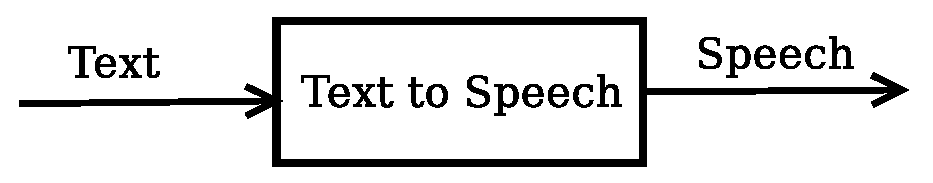
\includegraphics[scale=0.35]{figures/tts.eps}
\caption{Text to speech synthesis process}
\label{fig:ttsBlock}
\end{figure}

\subsubsection{HMM-based speech synthesis}
\label{ssec:hmm}
Hidden Markov Models (HMMs) can be used to model any time series. HMM tool kit (HTK) developed by Microsoft and Cambridge University is used to build HMMs. Initially HTK was
designed for building HMM-based speech processing tools, in particular recognizers. As 
shown in the picture above, there are two major processing stages involved. Firstly, the HTK training tools are used to estimate the parameters of a set of HMMs using training
utterances and their associated transcriptions. Secondly, unknown utterances are
transcribed using the HTK recognition tools.

\begin{figure}[h]
\centering
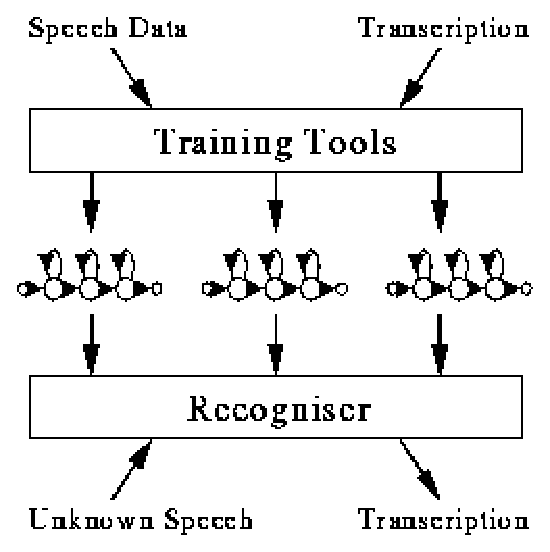
\includegraphics[scale=0.45]{figures/htk_overview.eps}
\caption{Overview of HTK}
\label{fig:htkOverview}
\end{figure}



The complete process of HMM-based speech synthesis system, shortly called as HTS 
(H-Triple-S) for a phoneme-level system is explained in the Algorithm \ref{algo:hts}.

\begin{algorithm}[!th]
\caption{Steps for text-to-speech using HTS }
\label{algo:hts}
\begin{algorithmic}[1]

\STATE  \textbf{Input:} Sentence(s) as text \\
\textbf{Output:} Synthesised speech
\STATE Prepare the speech corpus.
\STATE Pre-process the text data.
\STATE Segmentation and labelling of audio segments in corpus.
\STATE Manual correction of segmentation.
\STATE Preprocessing to get the phoneme labels.
\STATE Model training in HMM Training phase.
\STATE Verification of trained models.
\STATE HMM synthesis phase.
\end{algorithmic}
\end{algorithm}

\section{Evaluation Measures}
\label{sec:evalMeasures}
The first process of this project are image processing which analysis the image sequence
of climatic conditions and creates a weather report as text document with the location, direction, and speed of the cyclones. The accuracy of 
\begin{itemize}
\item the cyclone location
\item the direction of the cyclone movement
\item the speed of the cyclone movement
\item identifying the near-by or next hit areas in terms of city names
\end{itemize} are to be evaluated. This can be done by comparing the manually prepared report and the report generated by the automated process for the validation image set.

The second part of the project is to generate the synthesised voice from the text report. The synthesised voice has to be evaluated for 
\begin{itemize} 
\item intelligibility and 
\item naturalness.
\end{itemize} 
This can be evaluated by a measure called "Mean Opinion Score" (MOS) \cite{mos}.
This score is calculated by playing the natural human speech and the synthesised speech alternatively to a set of naive speakers and asking them to give scores in the scale of 1 to 5 to measure the intelligibility and naturalness of the synthesised speech. The scale of 1 to 5 has the standard meaning as given below.
\begin{table}[h]
\centering
\begin{tabular}{|c|l|l|}
\hline 
{\bf MOS	} & {\bf Quality } & {\bf Impairment} \\
\hline
5 & Excellent	& Imperceptible \\
4	& Good	& Perceptible but not annoying \\
3	& Fair	& Slightly annoying \\
2	& Poor	& Annoying \\
1	& Bad	& Very annoying \\ 
\hline 
\end{tabular}
\vspace{2mm}
\caption{Mean opinion score (MOS)}
\label{tab:mosDefn}
\end{table}

\subsection{Result of TTS}
\label{ssec:ttsResults}

The synthesized sentences are played along with the human spoken to 10 different naive listeners and they are asked to evaluate the sentences based on MOS in the scale of 5 as shown in the Table \ref{tab:mosDefn}. The average MOS of 3.4 out of 5 explains that the synthesized voices are intelligible with certain amount of naturalness in it. 

\subsection{Result of Image processing and NLG }
\label{ssec:imgResults}

The trajectory of the cyclone is formed by the movement of its eye. The correctness of the target cities and the cities reported as to be encountered in the cyclone path are verified manually. 

As per the reference to the NLG papers from the literature, the evaluation of generated weather reports is based on the questionnaire (Figure \ref{fig:questionare}) evaluated by different subjects. 

\begin{figure}[h!tb]
\centering
\includegraphics[scale=0.55]{figures/questionnare.png}
\caption{Sample questionnaire}
\label{fig:questionare}
\end{figure}

We chose the conversational English language to generate the report. So for the comparison and evaluation of the proposed system we used the manually written text reports in the telegraphic-weatherese format as mentioned in \cite{forecast} and \cite{Reiter}. The telegraphic-human generated sentences and the system generated sentences are shuffled and given to the users and are asked to evaluate the best understandable sentence. The proposed system in conversational format is evaluated as the better system.

\clearpage 

\bibliographystyle{IEEEtranS}
\bibliography{refs}


\end{document}
